% Convergence driver -- case_conv.py.
% 1D single Fourier mode on a PERIODIC domain (no boundary error):
%   T(x,0) = T0 + A sin(2 pi x/L).
% The harness sweeps the grid (dt capped at the acoustic CFL on coarse grids)
% for the spatial order, and sweeps dt on a fixed grid for the temporal order.
% Expected: 2-point central flux -> slope 2 in space; TVD-RK3 -> slope 3 in time.
%
% Compile:  pdflatex setup_conv.tex
\documentclass[border=6pt]{standalone}
\usepackage{amsmath}
\usepackage{tikz}
\usepackage{pgfplots}
\pgfplotsset{compat=1.18}
\usetikzlibrary{arrows.meta}

\definecolor{coldc}{RGB}{46,86,149}
\definecolor{hotc}{RGB}{171,57,52}
\definecolor{inkc}{RGB}{30,30,30}
\definecolor{accc}{RGB}{31,107,99}

\begin{document}
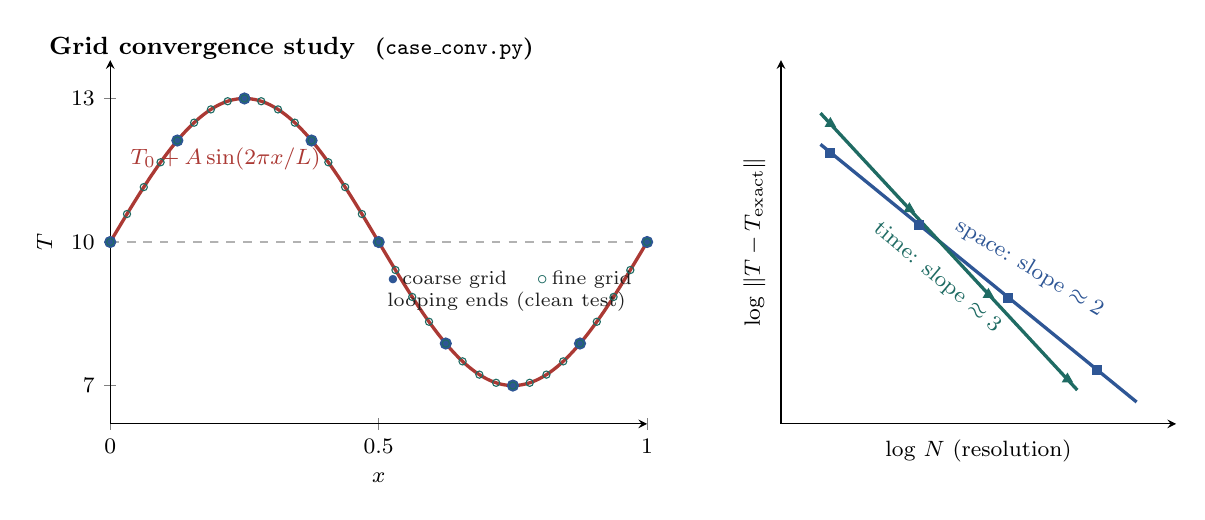
\begin{tikzpicture}[>=Stealth, font=\footnotesize]
% MAIN: the periodic mode, sampled on a coarse and a fine grid
\begin{axis}[
  name=mode, width=8.4cm, height=6.2cm,
  xlabel={$x$}, ylabel={$T$},
  xmin=0, xmax=1, ymin=6.2, ymax=13.8, axis lines=left, samples=200,
  xtick={0,0.5,1}, ytick={7,10,13}, enlargelimits=false, clip=false,
]
  \addplot[gray!60, dashed, thick, domain=0:1] {10};
  % continuous mode
  \addplot[hotc, very thick, domain=0:1] {10 + 3*sin(deg(2*pi*x))};
  % coarse sampling (few points)
  \addplot[only marks, mark=*, coldc, mark size=2.0pt, samples=9, domain=0:1]
    {10 + 3*sin(deg(2*pi*x))};
  % fine sampling (many points)
  \addplot[only marks, mark=o, accc, mark size=1.3pt, samples=33, domain=0:1]
    {10 + 3*sin(deg(2*pi*x))};
  \node[hotc, anchor=south west] at (axis cs:0.02,11.3) {$T_0+A\sin(2\pi x/L)$};
  \node[anchor=north east, align=left, font=\scriptsize, inkc]
    at (axis cs:0.99,9.6)
    {\textcolor{coldc}{$\bullet$}\,coarse grid \quad
     \textcolor{accc}{$\circ$}\,fine grid\\
     looping ends (clean test)};
\end{axis}

% INSET: expected log-log convergence (slope-2 space, slope-3 time guides)
\begin{axis}[
  name=conv, at={(mode.east)}, anchor=west, xshift=1.7cm,
  width=6.6cm, height=6.2cm,
  xlabel={$\log\,N$ (resolution)}, ylabel={$\log\,\|T-T_{\text{exact}}\|$},
  xmin=0, xmax=4, ymin=-7, ymax=0, axis lines=left,
  xtick=\empty, ytick=\empty, enlargelimits=false, clip=false,
]
  % slope -2 reference (spatial, central difference)
  \addplot[coldc, very thick, domain=0.4:3.6] {-1.0 - 1.55*x};
  \node[coldc, anchor=south west, rotate=-31] at (axis cs:1.6,-3.4)
    {space: slope $\approx 2$};
  % slope -3 reference (temporal, TVD-RK3)
  \addplot[accc, very thick, domain=0.4:3.0] {-0.2 - 2.05*x};
  \node[accc, anchor=north east, rotate=-40] at (axis cs:2.4,-5.0)
    {time: slope $\approx 3$};
  % markers along each line
  \addplot[only marks, mark=square*, coldc, mark size=1.6pt]
    coordinates {(0.5,-1.78)(1.4,-3.17)(2.3,-4.57)(3.2,-5.96)};
  \addplot[only marks, mark=triangle*, accc, mark size=2.0pt]
    coordinates {(0.5,-1.22)(1.3,-2.86)(2.1,-4.51)(2.9,-6.14)};
\end{axis}

\node[font=\bfseries\small, anchor=south west] at (-0.9,4.5)
  {Grid convergence study \ \footnotesize(\texttt{case\_conv.py})};
\end{tikzpicture}
\end{document}
